\documentclass[../../main/main.tex]{subfiles}
\graphicspath{{./figures/}}

\makeatletter
\renewcommand{\@chapapp}{Chimie -- chapitre}
\makeatother

\toggletrue{student}
% \HideSolutionstrue
% \toggletrue{corrige}
% \renewcommand{\mycol}{black}
\renewcommand{\mycol}{gray}

\begin{document}
\setcounter{chapter}{2}

\chapter{\cswitch{Correction du TD}{TD~: Cin\'etique chimique}}

\section{Pour s'échauffer}
\subsection{Énergie d'activation et constante de vitesse}
\QR{%
	Calculer l'énergie d'activation de la conversion du cyclopropane en
	propène à partir des données suivantes~:
	\begin{center}
		\begin{tabular}{lcccc}
			\toprule
			$T(\si{K})$      &
			750              & 800          & 850          & 900        \\
			\midrule
			$k(\si{s^{-1}})$ &
			\num{1.8e-4}     & \num{2.7e-3} & \num{3.0e-2} & \num{0.26} \\
			\bottomrule
		\end{tabular}
	\end{center}
}{%
	On sait que $k(T) = A\exr^{-E_a/RT}$. Avec une succession de
	températures, on peut tracer $\ln(k(T)) = f(1/T)$ afin de vérifier la
	loi~:

	\begin{minipage}{0.45\linewidth}
		\[\ln(k(T)) = \ln A - \frac{E_a}{R}\times \frac{1}{T}\]
		On trouve une régression de $r^2 = \num{0.99999}$, avec $\ln A =
			\num{35.0}$ et
		\begin{gather*}
			- \frac{E_a}{R} = \SI{-32.7e3}{K}\\
			\Leftrightarrow
			\boxed{E_a = \SI{2.7e5}{J.mol^{-1}}}
		\end{gather*}
	\end{minipage}
	\begin{minipage}{0.55\linewidth}
		\begin{center}
			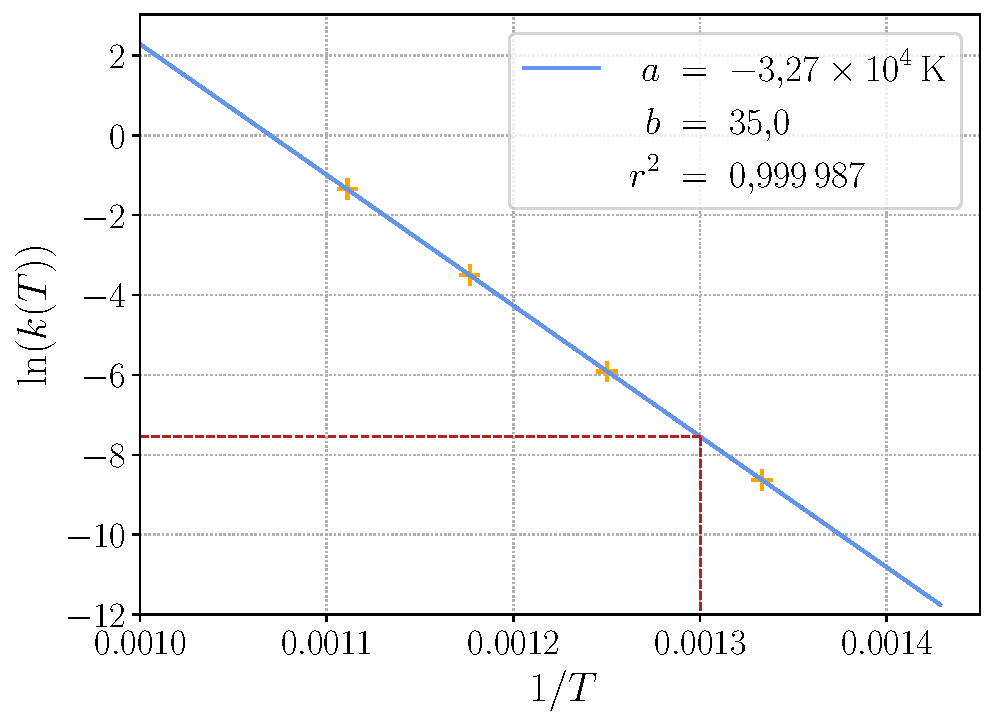
\includegraphics[width=\linewidth]{exo1_lnk}
		\end{center}
	\end{minipage}
}

\QR{%
	Quelle est la valeur de la constante de vitesse à
	\SI{500}{\degreeCelsius}~?
}{%
	Avec la régression linéaire précédente, on doit trouver la valeur de
	$\ln(k)$ avec $T = \SI{773}{K}$, c'est-à-dire $1/T =
		\SI{1.30e-3}{K^{-1}}$~: par lecture graphique, on trouve $\ln(k) =
		-\num{7.51}$, d'où
	\[\boxed{k(\SI{500}{\degreeCelsius}) = \SI{5.5e-4}{s^{-1}}}\]
}

\subsection{Utilisation du temps de demi-réaction}
\enonce{%
	Soit la réaction
	\[\ce{A -> B + C}\]
}
\QR{%
	Déterminer son ordre sachant que lorsqu'on multiplie par 10 la concentration
	initiale de A, on divise le temps de demi-réaction par 10.
}{%
	D'après le cours, pour une réaction d'ordre 2 en A uniquement, on a $t_{1/2} =
		\frac{1}{ka[\ce{A}]_0}$ avec $a$ le coefficient stœchiométrique du composé A.
	C'est la seule situation où augmenter la concentration baisse le temps de
	demi-réaction~: l'ordre 0 a un $t_{1/2} \propto [\ce{A}]_0$, et l'ordre 1 ne
	dépend pas de $[\ce{A}]_0$~: on a donc une \textbf{réaction d'ordre 2 en A}.
}

\resetQ
\section{Utilisation de la méthode intégrale}
\enonce{%
	À température élevée et en phase gazeuse, le buta-1,3-diène se dimérise en
	4-vinylcyclohexène suivant la réaction totale d'équation
	\[\ce{2C4H6\gaz{} = C8H12\gaz{}}\]
	Afin d'étudier cette réaction, une certaine quantité de buta-1,3-diène est
	introduite dans un récipient de volume $V$ constant, maintenu à température
	constante $T = \SI{326}{K}$. On mesure alors la pression partielle en butadiène
	$p_B$ dans le récipient en fonction du temps~:
	\begin{center}
		\begin{tabular}{lcccccccccccc}
			\toprule
			$t(\si{min})$   &
			0               & \num{3.25}  & \num{8.02}  & \num{12.18} & \num{17.3}  & \num{24.55} &
			\num{33.0}      & \num{43.0}  & \num{55.08} & \num{68.05} & \num{90.1}  &
			\num{119}                                                                               \\
			\midrule
			$p_B(\si{bar})$ &
			\num{0.843}     & \num{0.807} & \num{0.756} & \num{0.715} & \num{0.670} &
			\num{0.615}     & \num{0.565} & \num{0.520} & \num{0.465} & \num{0.423} &
			\num{0.366}     & \num{0.311}                                                           \\
			\bottomrule
		\end{tabular}
	\end{center}
}

\QR{%
	Montrer, en utilisant la loi des gaz parfaits, que la connaissance de
	la pression initiale $p_B$ et de la température $T$ suffit pour calculer
	la concentration initiale $c_B$ en buta-1,3-diène.
}{%
	On utilise la loi du gaz parfait~:
	\begin{gather*}
		\frac{n_B}{V} = \frac{p_B}{RT}
		\Leftrightarrow
		\boxed{c_B = \frac{p_{B,0}}{RT}}
		\qavec
		\left\{
		\begin{array}{rcl}
			p_{B,0} & = & \SI{0.843}{bar} = \SI{8.43e-4}{Pa} \\
			R       & = & \SI{8.314}{J.mol^{-1}.K^{-1}}      \\
			T       & = & \SI{326}{K}
		\end{array}
		\right.\\
		\mathrm{A.N.~:}\quad
		\boxed{c_B = \SI{31.5}{mol.m^{-3}}}
		\Leftrightarrow
		\boxed{c_B = \SI{31.5e-3}{mol.L^{-1}}}
	\end{gather*}
	Faites bien attention aux unités utilisées dans l'application numérique,
	qui viennent ici de celles de l'équation d'état des gaz parfait.
}

\QR{%
Montrer que les résultats sont compatibles avec une cinétique d'ordre
2. Déterminer alors la constante de vitesse à cette température.
}{%
Faisons l'hypothèse d'une cinétique d'ordre 2. Pour simplifier les
écritures, notons $\ce{X} = \ce{C4H6}$. Une loi de vitesse d'ordre 2 en
X signifie qu'elle s'écrit
\[
	v = k[\ce{X}]^2
	\qquad\text{mais on a aussi}\qquad
	v = - \frac{1}{2} \dv{[\ce{X}]}{t}
\]
grâce au lien entre vitesse de disparition d'un réactif et vitesse d'une
réaction. Comme dans le cours, cela se traduit par
\begin{gather*}
	- \frac{1}{2} \dv{[\ce{X}]}{t} = k[\ce{X}]^2
	\Leftrightarrow
	\frac{\mathrm{d} [\ce{X}]}{[\ce{X}]^2} = -2k\dt
	\Leftrightarrow
	- \frac{1}{[\ce{X}]} = -2kt + K
\end{gather*}
en primitivant de part et d'autre. On trouve $K$ par la condition
initiale~: $[\ce{X}](t=0) = c_{B,0}$. On a donc \fbox{$K = -1/c_{B,0}$}
et finalement
\[\boxed{ \frac{1}{[\ce{X}]} = \frac{1}{c_{B,0}} + 2kt}\]
Pour vérifier cet ordre 2, il suffit donc de tracer

\begin{minipage}{0.45\linewidth}
	\[  y = ax + b
		\qavec
		\left\{
		\begin{array}{rcl}
			y         & = & \frac{1}{[\ce{X}]} \\\relax
			[\ce{X}] & = & \frac{p_B}{RT}      \\
			a         & = & 2k                  \\
			x         & = & t                   \\
			b         & = & \frac{1}{c_{B,0}}
		\end{array}
		\right.
	\]
\end{minipage}
\begin{minipage}{0.55\linewidth}
	\begin{center}
		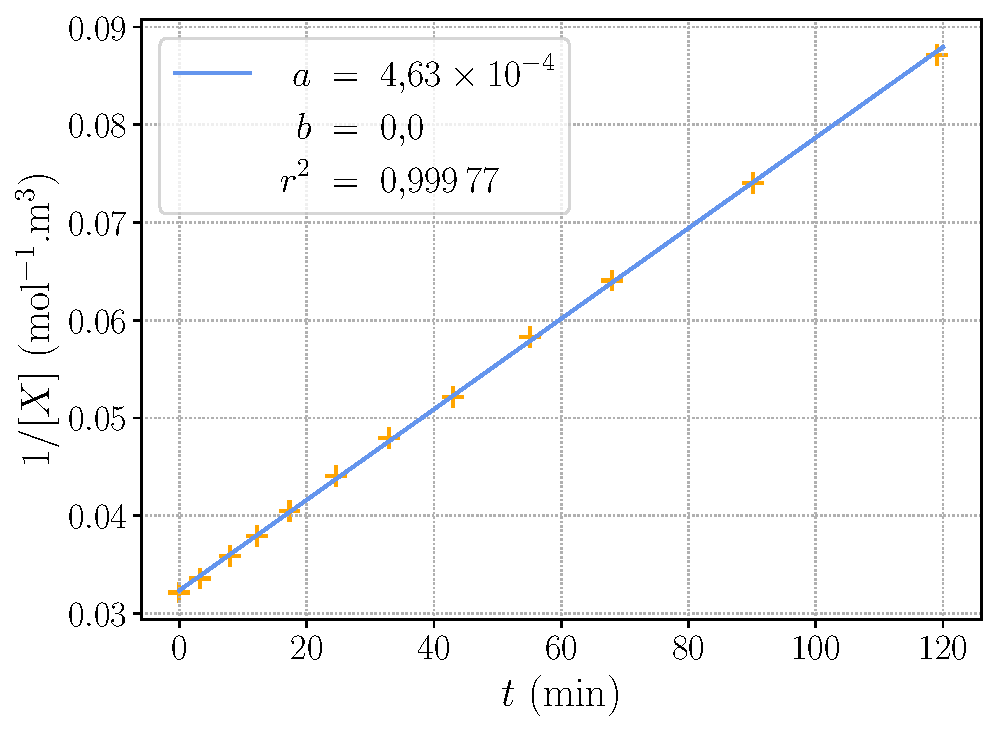
\includegraphics[width=\linewidth]{exo2_x}
	\end{center}
\end{minipage}
On observe que la régression passe bien par tous les points, et on
trouve également $r^2 = \num{0.9997}$, validant l'ordre 2. Le
coefficient directeur valant $2k$, on trouve finalement
\[\boxed{k =
	\SI{2.32e-4}{mol^{-1}.m^3.min^{-1}}
	=
	\SI{2.32e-1}{mol^{-1}.L.min^{-1}}
	}
\]
}

\QR{%
	Déterminer le temps de demi-réaction du système précédent.
}{%
	Pour un système d'ordre 2, on a $t_{1/2} = \frac{1}{ka[\ce{A}]_0}$ avec
	$a$ le coefficient stœchiométrique arithmétique de l'élément A. Ici, le
	coefficient stœchiométrique du butadiène est 2, et on a donc
	\begin{gather*}
		t_{1/2} = \frac{1}{2kc_{B,0}}
		\Leftrightarrow
		\boxed{t_{1/2} = \SI{70.0}{min}}
	\end{gather*}
}
\QR{%
	On admet souvent qu'une réaction est pratiquement terminée lorsque au
	moins 99\% du réactif limitant a été consommé. Déterminer la durée
	d'évolution du système précédent~; exprimer cette durée en fonction du
	temps de demi-réaction.
}{%
	On cherche donc $t_{99}$ tel qu'il ne reste que 1\% de $c_{B,0}$,
	c'est-à-dire~:
	\begin{gather*}
		[\ce{X}](t = t_{99}) = \frac{1}{100}c_{B,0}
		\Leftrightarrow
		\frac{100}{c_{B,0}} = \frac{1}{c_{B,0}} + 2kt_{99}
		\Leftrightarrow
		t_{99} = \frac{1}{2k}\times \frac{99}{c_{B,0}}\\
		\Leftrightarrow
		\boxed{
			t_{99} = 99t_{1/2}
		}
		\qdonc
		\boxed{t_{99} = \SI{6930}{min} = \SI{115.5}{h} = \SI{4.8125}{jours}}
	\end{gather*}
}

\resetQ
\section{Utilisation de la méthode différentielle}
\label{sec:mtdiff}
\enonce{%
  La réaction étudiée est l'oxydation des ions iodure par les ions ferriques
Fe(III). Les couples d'oxydoréduction mis en jeu sont les couples
$\ce{I2}/\ce{I-}$ et $\ce{Fe^{3+}}/\ce{Fe^{2+}}$, toutes les espèces étant
dissoutes dans l'eau.
}

\QR{%
  Écrire l'équation-bilan de l'oxydation des ions iodure par les ions
        fer (III), en affectant les espèces du fer du nombre stœchiométrique 1.
        Si la concentration d'ions iodure passe de $c_0$ à $c_0 - x$ entre 0 et
        $t$, comment définit-on par rapport à $x$ la vitesse volumique de la
        réaction~?
}{%
        \begin{tcb}(data)<lfnt>{Données}
            Même sans connaître le principe de l'oxydo-réduction, la réaction
            étudiée met en contact les ions iodure, donc $\ce{I-}$, et les ions
            fer III, donc $\ce{Fe^{3+}}$. Par déduction les produits sont les
            autres composés cités, c'est-à-dire $\ce{I2}$ et $\ce{Fe^{2+}}$. La
            manière la plus simple de l'équilibrer serait avec des nombres
            entiers et notamment $2$ devant chaque élément sauf $\ce{I2}$, mais
            on nous demande de l'écrire avec un nombre stœchiométrique de $1$
            devant les espèces du fer.
        \end{tcb}
        En tant qu'équation-bilan et donc qu'équation, il suffit de diviser
        chaque côté par 2 pour obtenir~:
        \begin{tcb}(rslt)<lfnt>{Résultat}
            \[\ce{Fe^{2+}\aqu{} + I^{-}\aqu{} = Fe^{2+}\aqu{} +
        1/2I2\aqu{}}\]
        \end{tcb}
        Il n'est en effet pas choquant d'avoir des coefficients stœchiométriques
        qui ne sont pas entiers dans une équation-bilan. \bigbreak
        \begin{tcb}(rapp)<lfnt>{Outil}
            Avec le cours, on sait que
            \[v = \frac{1}{\nu_i} \dv{[\ce{X}_i]}{t}\]
            pour X$_i$ un élément de l'équation-bilan
            \[0 = \sum_{i} \nu_i\ce{X}_i\]
        \end{tcb}
        \begin{tcb}(appl)<lfnt>{Application}
            Si on veut exprimer $v$ en fonction de la concentration en ions iodure,
            on a donc
            \begin{gather*}
                v = \frac{1}{-1} \dv{[\ce{I-}]}{t}
                = - \dv{c_0 - x}{}
                \Leftrightarrow
                \boxed{v = \dv{x}{t}}
            \end{gather*}
            étant donné que $c_0$ est une constante.
        \end{tcb}
}

\QR{%
  On suppose une cinétique avec ordre, de constante de vitesse $k$~; on
  note $a$ l'ordre partiel par rapport aux ions fer (III) et $b$ l'ordre
  partiel par rapport aux ions iodure. Comment s'écrit la vitesse $v$~?
  Quelle est alors l'unité usuelle de $k$ (au besoin en fonction de $a$ et
  de $b$)~?
}{%
Dans le cours, on a
  \begin{tcb}(tool)<lfnt>{Outil}
      %\color{BlueViolet!60!black}
      Une réaction $a\ce{A} + b\ce{B} = c\ce{C} + d\ce{D}$ a une loi
      de vitesse admettant un ordre si elle s'écrit
      \[v = k[\ce{A}]^{\alpha}[\ce{B}]^{\beta}\]
      avec $\alpha$ l'ordre partiel par rapport au réactif A et $\beta$
      l'ordre partiel par rapport au réactif B.
  \end{tcb}
  \begin{tcb}(prop)<lfnt>{Résultat}
      Ici, les réactifs sont les ions fer III et les ions iodure, donc la
      vitesse s'écrirait donc
      \[
          \boxed{
              v = k [\ce{Fe^{3+}}]^a[\ce{I^{-}}]^b
          }
      \]
  \end{tcb}
  \begin{tcb}(appl)<lfnt>{Application}
      On trouve l'unité de $k$ en étudiant celles des termes en jeu dans
      l'équation~:
      \[\si{mol.L^{-1}.s^{-1}} = [k]\times (\si{mol.L^{-1}})^{a+b}\]
      donc la dimension de $k$ est
      \fbox{$(\si{mol.L^{-1}})^{1-a-b}\si{s^{-1}}$}.
  \end{tcb}
}
\QR{%
  À la date $t$ après le mélange d'une solution d'iodure de potassium
  avec une solution ferrique, on prélève à la pipette \SI{5}{mL} de
  solution et on dilue 10 fois avant de procéder à un dosage de la
  quantité d'iode formée. Justifier l'intérêt cinétique de cette dilution.
}{%
Dans la dernière partie du cours, nous avons introduit le concept du
dosage par titrage, et exposé la nécessité de \textbf{ralentir la
réaction} pour qu'un volume de solution prélevé à un instant $t$ mais
dosé par méthode chimique à un instant ultérieur ait une évolution
négligeable entre ces deux instants~: cette pratique s'appelle la
\textbf{trempe chimique}, et une des manières de réaliser une trempe
chimique est de fortement diluer la solution prélevée. En effet, la
vitesse étant reliée à la concentration en les réactifs (pour une
réaction admettant un ordre), on peut «~geler~» l'état de la réaction en
augmentant le volume du solvant et donc en réduisant la concentration
des éléments.
}

\QR{%
  Les résultats d'une série de mesures sont présentés ci-dessous, $x$ se
  rapportant à la quantité d'ions iodure qui ont été oxydés dans le milieu
  réactionnel à la date du prélèvement.
  \begin{center}
    \begin{tabular}{lccccc}
      \toprule
      $t(\si{s})$                 &
      60                          & 120 & 180 & 240 & 300 \\
      \midrule
      $x(\si{\micro mol.L^{-1}})$ &
      13                          & 25  & 36  & 46  & 55  \\
      \bottomrule
    \end{tabular}
  \end{center}
  Que représente la grandeur $x(t)/t$~? Pourquoi diminue-t-elle en cours
  de réaction~? Représenter graphiquement cette grandeur en fonction de
  $t$ à partir du tableau ci-dessus, avec en abscisse $t \in
    \SIrange{0}{300}{s}$~; en déduire une estimation de la valeur initiale
  $\left.\dv{x}{t}\right|_0$.
}{%
  \begin{minipage}{0.45\linewidth}
      \begin{center}
          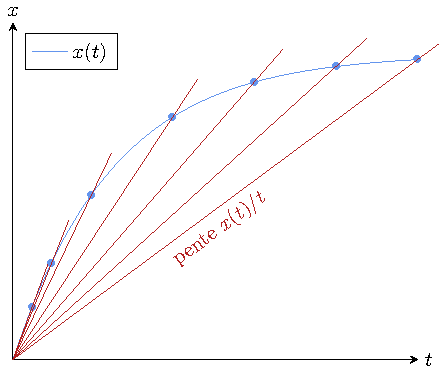
\includegraphics[width=\linewidth]{xtt}
      \end{center}
  \end{minipage}
  \hfill
  \begin{minipage}{0.45\linewidth}
      On peut commencer par remarquer que $x(t)/t$ a la dimension d'une
      vitesse de réaction, en $\si{mol.L^{-1}.s^{-1}}$. Il faut ensuite
      remarquer que $x(t)/t = (x(t) - x(0))/(t-0)$ avec un avancement nul
      à $t=0$~; si $t$ est suffisamment petit, on a donc
      \[ \frac{x(t)}{t} \approx \left.\dv{x}{t}\right|_0\]
      et ainsi $x(t)/t$ est une approximation de la vitesse de la
      réaction~; c'est ce qu'on appelle l'approximation de la tangente par
      la sécante. En faisant la régression linéaire jusqu'en 0, on
      trouvera bien la vitesse en 0.
  \end{minipage}

  On réalise cette régression avec $y = x(t)/t$, $x = t$ et $b = v_0$,
  pour obtenir le résultat suivant~:
  \begin{minipage}{0.45\linewidth}
      On trouve alors, grâce à l'ordonnée à l'origine,
      \[\boxed{v_0 = \SI{2.25e-7}{mol.L^{-1}.s^{-1}}}\]
  \end{minipage}
  \begin{minipage}{0.55\linewidth}
      \begin{center}
          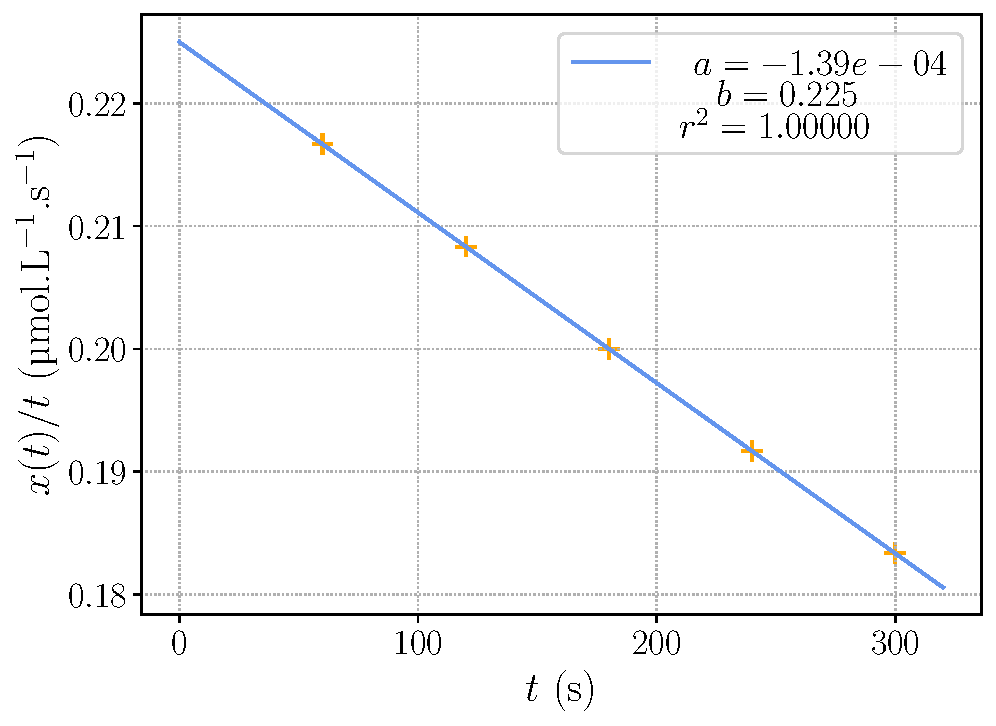
\includegraphics[width=\linewidth]{exo3_xtt}
      \end{center}
  \end{minipage}
}

\QR{%
  Grâce à la méthode précédente, on détermine les valeurs initiales de
  $\dv{x}{t}$ pour différentes concentrations initiales des deux réactifs.
  Quelques résultats sont présentés ci-dessous~:
  \begin{center}
    \begin{tabular}{lccccccc}
      \toprule
      $c_0 = [\ce{I-}]_0$                &
      $(\si{\micro mol.L^{-1}})$         &
      2                                  & 2          & 2          & 6  & 6  & 8   \\
      \midrule
      $[\ce{Fe^{3+}}]_0$              &
      $(\si{\micro mol.L^{-1}})$         &
      2                                  & 4          & 8          & 2  & 4  & 8   \\
      \midrule
      $\DS \eval{\dv{x}{t}}_{0}$ &
      $(\si{\micro mol.L^{-1}.s^{-1}})$  &
      \num{5.7}                          & \num{11.1} & \num{22.5} & 52 & 99 & 354 \\
      \bottomrule
    \end{tabular}
  \end{center}
  En déduire les valeurs de $a$ et $b$, supposées entières.
}{%
Pour déterminer les valeurs de $a$ et $b$, il faut utiliser des
        expériences dans lesquelles l'une des deux concentrations est fixe alors
        que l'autre non~: ça revient au même principe que la dégénérescence de
        l'ordre.\bigbreak
        Ici, dans les expériences 1, 2 et 3 par exemple, on a $[\ce{I-}]_0 =
        \cte$. Dans ce cas, à chaque fois on a
        \begin{gather*}
            v_{0,1} = k[\ce{Fe^{3+}}]_{0,1}{}^a [\ce{I-}]_0{}^b\\
            v_{0,2} = k[\ce{Fe^{3+}}]_{0,2}{}^a [\ce{I-}]_0{}^b\\
            v_{0,3} = k[\ce{Fe^{3+}}]_{0,3}{}^a [\ce{I-}]_0{}^b
        \end{gather*}
        et $v_0$ ne dépend que de la concentration en ions fer III. Comme on
        cherche des ordres partiels entier, on en déduit qu'il suffit d'étudier
        comment varie $v_0$ à une modification simple de la concentration
        initiale en ions fer III pour déduire l'ordre~: ici par exemple, en
        multipliant par $2$ cette concentration initiale, la vitesse est
        multipliée par environ 2 à chaque fois. Le seul ordre partiel $a$
        permettant cette relation est bien évidemment un ordre partiel égal à
        1~: on en déduit \fbox{$a = 1$}. \bigbreak
        De même, avec des expériences où la concentration initiale en ions fer
        III est fixe, par exemple pour les 1 et 4, on a une variation de $v_0$
        dépendante uniquement de la concentration initiale en ions iodure. Or,
        on remarque cette fois que multiplier par 3 cette concentration multiplie
        par 9 la vitesse initiale~: le seul ordre partiel entier qui permet que
        $3^b = 9$ est bien évidemment 2, et on en déduit \fbox{$b = 2$}.
}
\QR{%
  Déterminer la constante de vitesse $k$ définie à la question 2)~; on
        précisera la méthode suivie pour utiliser au mieux les données.
}{%
On pourrait mesurer $k$ en prenant $v_0/([\ce{Fe^{3+}}]_{0}{}\times
        [\ce{I-}]_0{}^2)$ à chaque fois et en faisant la moyenne, mais pour
        avoir la meilleure estimation avec ces données la régression linéaire
        est plus efficace~: les éventuelles variabilités de mesure se combinent
        toutes ensemble pour avoir une estimation combinée dépendante, plutôt
        qu'une estimation moyennée où les valeurs sont supposées indépendantes.
        Ainsi, on trace
        \begin{gather*}
            v_0 = f([\ce{Fe^{3+}}]_{0}{}\times [\ce{I-}]_0{}^2)
        \end{gather*}
        dont le coefficient directeur sera $k$.

        \begin{minipage}{0.45\linewidth}
            On trouve alors
            \begin{gather*}
                k = \SI{6.90e-1}{\micro mol^{-2}.L^2.s^{-1}}\\
                \Leftrightarrow
                \boxed{
                k = \SI{6.90e11}{mol^{-2}.L^2.s^{-1}}}
            \end{gather*}
        \end{minipage}
        \hfill
        \begin{minipage}{0.55\linewidth}
            \begin{center}
                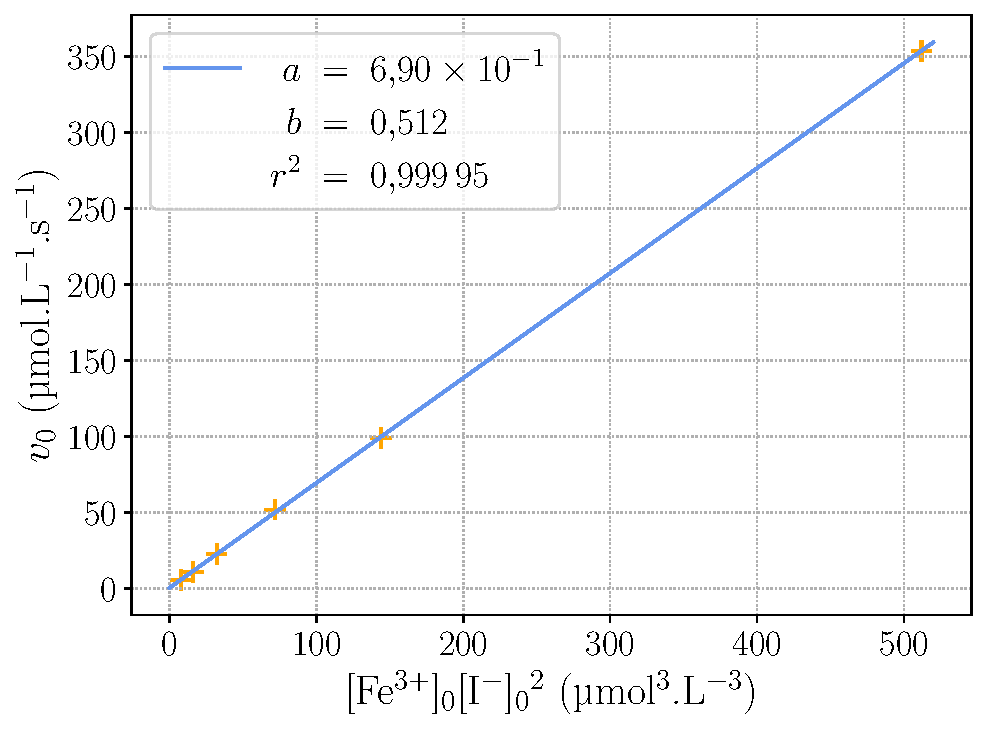
\includegraphics[width=\linewidth]{exo3_v0}
            \end{center}
        \end{minipage}
}
\QR{%
  Dans l'hypothèse d'un état initial ne contenant que les deux réactifs à la
  même concentration $c_0$, établier la relation littérale donnant $x(t)$ sous
  la forme~:
  \begin{center}
    «~expression en $(x,c_0)$ = expression en $(k,t)$~»
  \end{center}
  En déduire la dépendance entre le temps de demi-réaction $\tau$ et la
  concentration $c_0$.
}{%
  \begin{tcb}(data)<lfnt>{Données}
      Les conditions de cette question sont celles des proportions
      stœchiométriques introduites dans le cours~: en effet, comme les deux
      réactifs ont le même coefficient stœchiométrique, leurs deux
      concentrations à un instant $t$ valent $c_0 -x$. Ainsi, la vitesse de
      réaction s'écrit
      \begin{gather*}
          v = k (c_0 - x)(c_0-x)^2 = k(c_0-x)^3 = \dv{x}{t}
      \end{gather*}
  \end{tcb}
  \begin{tcb}(appl)<lfnt>{Calcul}
      en la reliant à la question 1). Comme pour l'ordre 2, on résout cette
      équation en séparant les différentielles~:
      \begin{gather}\label{eq:difftrois}
          \frac{\dd x}{(c_0 -x)^3} = k\dt
      \end{gather}
  \end{tcb}
  \begin{tcb}(tool)<lfnt>{Outil}
      On doit, de cette équation, en trouver une primitive. Pour effectuer ce
      raisonnement, il est plus simple de partir d'une forme simple à dériver
      qui donnerait celle à gauche du signe égal. Or, on sait que pour $u$ une
      fonction,
      \[(u^{\alpha})' = \alpha u' u^{\alpha-1}\]
      Donc si $\alpha = -2$, on aura $u^{-3}$ en dérivant, ce qui correspond à
      notre équation à nous. Cependant, il faut faire attention aux constantes
      et signes $\pm$ dans de telles situations~: calculons la dérivée en
      entier.
      \[(u^{-2})' = -2 u' u^{-3}\]
      Soit
      \begin{gather*}
          \left.\begin{array}{rcl}
                    u~: \Rb^+ & \rightarrow & \Rb^+\\
                  x & \mapsto & c_0 - x\\
          \end{array}\right.
          \Rightarrow
          \left.\begin{array}{rcl}
                  \dd u : \Rb^+ & \rightarrow & \Rb^+\\
                  x & \mapsto & -\dd x\\
          \end{array}\right.
      \end{gather*}
      On a donc
      \[\dd((c_0 -x)^{-2}) = -2 (-\dd x) (c_0 - x)^{-3}\]
      Et en prenant la primitive de chaque côté,
      \[\int\dd((c_0 -x)^{-2}) = \int -2 (-\dd x) (c_0 - x)^{-3}\]
  \end{tcb}
  \begin{tcb}(rslt)<lfnt>{Résultat}
      On peut donc résoudre l'équation différentielle \ref{eq:difftrois} par
      intégration, pour obtenir
      \begin{gather*}
          \frac{1}{(c_0 - x)^2} = 2kt + K
          \qet
          \frac{1}{c_0{}^2} = K
          \qdonc
          \boxed{
          \frac{1}{(c_0-x)^2} - \frac{1}{c_0{}^2} = 2kt}
      \end{gather*}
  \end{tcb}
  \begin{tcb}(defi)<lfnt>{Définition}
      Or, par définition, le temps de demi-réaction est le temps au bout
      duquel l'avancement est à la moitié de sa valeur finale,
      c'est-à-dire $x(\tau) = x_f/2$.
  \end{tcb}
  \begin{tcb}(appl)<lfnt>{Calcul}
      Ici, on trouve donc
      \begin{gather*}
          x(\tau) = \frac{c_0}{2}
          \Leftrightarrow
          \frac{1}{(c_0 - \frac{c_0}{2})^2} - \frac{1}{c_0{}^2} = 2k\tau
          \Leftrightarrow
          \frac{4}{c_0{}^2} - \frac{1}{c_0{}^2} = 2k\tau\\
      \end{gather*}
  \end{tcb}
  \begin{tcb}(rslt)<lfnt>{Résultat}
      Soit finalement
      \[\boxed{\tau = \frac{3}{2kc_0{}^2}}\]
  \end{tcb}
}


\resetQ
\section{Étude d'un mélange stœchiométrique}
\enonce{%
  On étudie à \SI{25}{\degreeCelsius} l'action d'une solution de soude diluée sur
  le bromoéthane~; la réaction totale a pour équation~:
  \[\ce{CH3CH2Br + HO^{-} <=> CH3CH2OH + Br^{-}}\]
  On utilise des mélanges stœchiométriques en bromoéthane et en ion hydroxyde.
  Soit $c_0$ la concentration initiale commune des deux réactifs. Le tableau
  ci-dessous donne les temps de demi-réaction pour différentes valeurs de $c_0$.
  \begin{center}
    \begin{tabular}{lccccc}
      \toprule
      $c_0 (\si{mmol.L^{-1}})$ &
      10                       & 25  & 50  & 75  & 100 \\
      \midrule
      $\tau_{1/2} (\si{min})$  &
      1100                     & 445 & 220 & 150 & 110 \\
      \bottomrule
    \end{tabular}
  \end{center}
}

\QR{%
  Démontrer que ces données sont compatibles avec une réaction d'ordre
  partiel 1 par rapport à chacun des réactifs.
}{%
Si la réaction est d'ordre 1 par rapport à chacun des réactifs, cela
veut dire qu'elle s'écrit
\[v = k [\ce{CH3CH2Br}][\ce{HO-}]\]
Leurs coefficients stœchiométriques sont égaux à -1, ce qui veut dire
que chacun de ces réactifs a une concentration $c(t) = c_0 - \xi(t)$ à
chaque instant~; ainsi
\[v = k c(t)^2\]
Cette réaction est équivalente à une réaction d'ordre 2 par rapport à un
unique réactif, dont le temps de demi-réaction est
\[\tau_{1/2} = \frac{1}{kc_0}\]
Pour vérifier que les données sont compatibles avec cette relation, on
trace $\tau_{1/2} = f(1/c_0)$ en traçant
\[y = ax
    \qavec
    \left\{
        \begin{array}{rcl}
            y & = & t_{1/2}\\
            a & = & 1/k\\
            x & = & 1/c_0
        \end{array}
    \right.
\]
\begin{minipage}{0.45\linewidth}
    On trouve bien ici une droite avec un coefficient de corrélation
    $r^2 = \num{0.99997}$, confirmant que l'\textbf{ordre global} est
    compatible avec 2.
    \begin{tcb}(impo){Attention}
        Cette démarche ne prouve en rien que les ordres partiels sont
        chacun de 1~: ils pourraient être de 1/2 et 3/2 respectivement.
    \end{tcb}
\end{minipage}
\hfill
\begin{minipage}{0.55\linewidth}
    \begin{center}
        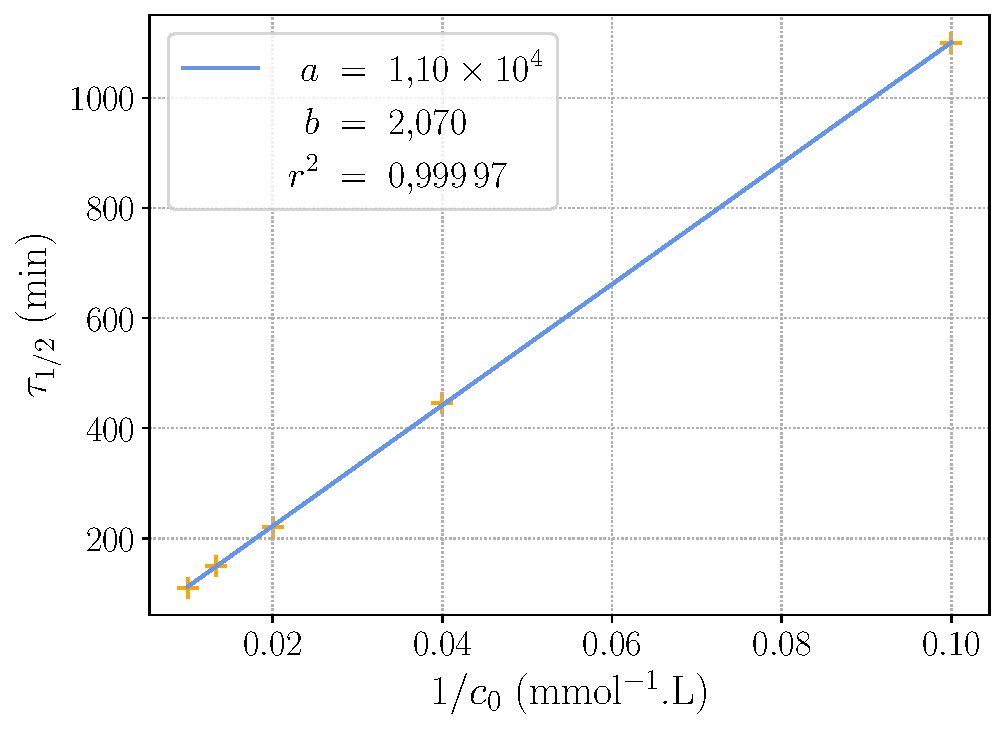
\includegraphics[width=\linewidth]{exo4_tab}
    \end{center}
\end{minipage}
}

\QR{%
  Déterminer la constante de vitesse de la réaction.
}{%
Comme déterminé dans la régression linéaire, le coefficient directeur
de la droite est l'inverse de la constante de vitesse. On trouve donc
\[\boxed{k = \SI{9.10e-5}{mmol^{-1}.L.min^{-1}} =
\SI{9.10e-2}{mol^{-1}.L.min^{-1}}}\]
}

\resetQ
\section{Méthode des vitesses initiales}
\enonce{%
  Le chlorure d'hydrogène (B) réagit sur le cyclohexène (A) avec formation de
chlorocyclohexane (C), selon la réaction~:
\[\ce{C6H10 + HCl \longrightarrow C6H11Cl}
  \quad
  \text{schématisée par}
  \quad
  \ce{A} + \ce{B} \longrightarrow \ce{C}
\]
On réalise une série d'expériences à \SI{25}{\degreeCelsius}, où l'on mesure la
vitesse initiale $v_0$ de la réaction en fonction des concentrations molaires
initiales $[\ce{A}]_0$ en cyclohexène et $[\ce{B}]_0$ en chlorure d'hydrogène
dans le milieu réactionnel. Le volume du mélange est constant et égal à
\SI{1}{L}. Les résultats sont rassemblés dans le tableau ci-dessous~:
\begin{center}
  \begin{tabular}{lcccc}
    \toprule
    Expérience                       &
    1                                & 2           & 3           & 4           \\
    \midrule
    $[\ce{A}]_0$ ($\si{mol.L^{-1}}$) &
    \num{0.470}                      & \num{0.470} & \num{0.470} & \num{0.313} \\
    $[\ce{B}]_0$ ($\si{mol.L^{-1}}$)   &
    \num{0.235}                      & \num{0.328} & \num{0.448} & \num{0.448} \\
    $v_0$ ($\SI{e-9}{mol.s^{-1}}$)     &
    \num{15.7}                       & \num{30.6}  & \num{57.1}  & \num{38.0}  \\
    \bottomrule
  \end{tabular}
\end{center}
}

\QR{%
  On désigne par $p$ et $q$ les ordres partiels initiaux de la réaction
  par rapport au cyclohexène (A) et au chlorure d'hydrogène (B). Exprimer
  la loi de vitesse initiale de cette réaction en fonction de $p$ et $q$.
}{%
Par définition,
\[ v_0 = k[\ce{A}]_0{}^p[\ce{B}]_0{}^q\]
}

\QR{%
  Déterminer $p$.
}{%
  Comme dans l'exercice~\ref{sec:mtdiff}, il suffit de trouver deux expériences où
  $[\ce{B}]_0$ est constante pour voir comment $v_0$ varie par
  multiplication de $[\ce{A}]_0$. Ici, dans les expériences 3 et 4,
  $[\ce{B}]_0 = \SI{0.448}{mol.L^{-1}}$. On a donc
  \begin{gather*}
      \left\{
          \begin{array}{rcl}
              v_{0,3} & = & k[\ce{B}]_0{}^q\times [\ce{A}]_{0,3}{}^p\\
              v_{0,4} & = & k[\ce{B}]_0{}^q\times [\ce{A}]_{0,4}{}^p
          \end{array}
      \right.
      \Leftrightarrow
      \frac{v_{0,3}}{v_{0,4}} = \left(
          \frac{[\ce{A}]_{0,3}}{[\ce{A}]_{0,4}}\right)^p\\
      \Leftrightarrow
      \boxed{
      p = \frac{\ln(v_{0,3}/v_{0,4})}{\ln([\ce{A}]_{0,3}/[\ce{A}]_{0,4})}
      }\\
      \mathrm{A.N.~:}\quad
      \boxed{p \approx 1}
  \end{gather*}
  On en conclut que \fbox{$p = 1$}, en supposant l'ordre entier.
}

\QR{%
  Déterminer $q$~; en déduire l'ordre global de la réaction.
}{%
On fait de même avec les expériences 1 et 2 par exemple, où cette fois
c'est $[\ce{A}]_0$ qui est constante. On trouve alors
\begin{gather*}
    \boxed{
    q = \frac{\ln(v_{0,1}/v_{0,2})}{\ln([\ce{B}]_{0,1}/[\ce{B}]_{0,2})}
    }\\
    \mathrm{A.N.~:}\quad
    \boxed{q \approx 2}
\end{gather*}
On en conclut que \fbox{$q = 2$}, en supposant l'ordre entier. L'ordre
global, défini par $p+q$, est donc \fbox{$p+q = 3$}.
}
\QR{%
  Calculer la constante cinétique de la réaction.
}{%
Pour plus de précision, on peut tracer une régression linéaire de $v_0
= f([\ce{A}]_0[\ce{B}]_0{}^2)$ avec
\[y = ax
    \qavec
    \left\{
        \begin{array}{rcl}
            y & = & v_0\\
            a & = & k\\
            x & = & [\ce{A}]_0[\ce{B}]_0{}^2
        \end{array}
    \right.
\]
\begin{minipage}{0.45\linewidth}
    On trouve bien ici une droite avec un coefficient de corrélation
    $r^2 = \num{0.99997}$, confirmant que l'\textbf{ordre global} est
    compatible avec 3. Le coefficient directeur donne directement $k$,
    et on a
    \[\boxed{k = \SI{6.05e-7}{mol^{-2}.L^2.s^{-1}}}\]
\end{minipage}
\hfill
\begin{minipage}{0.45\linewidth}
    \begin{center}
        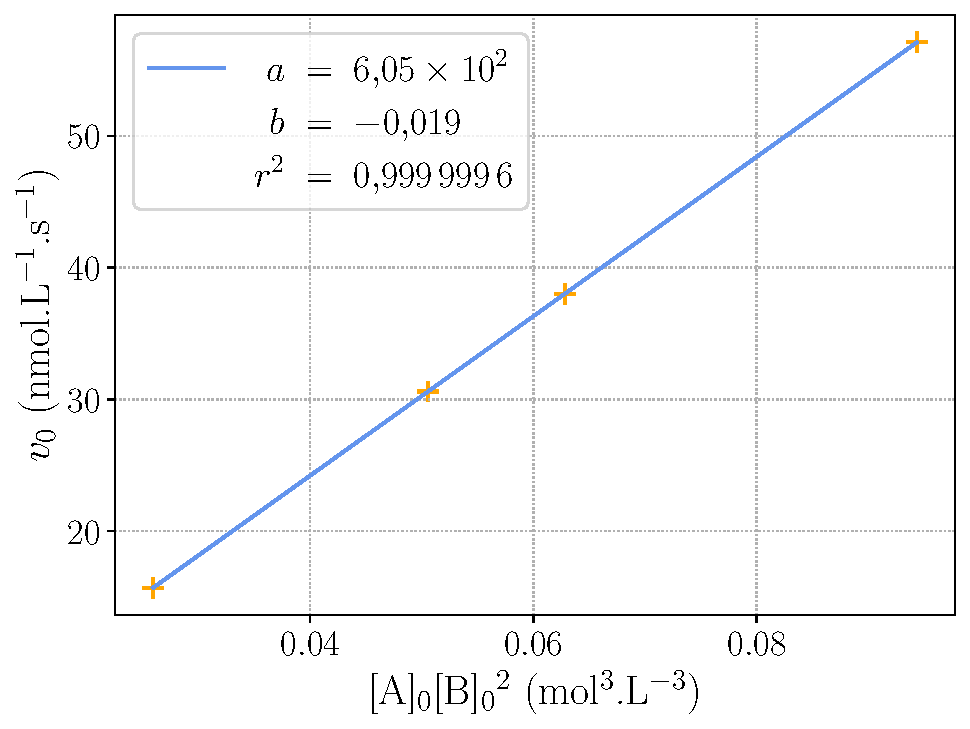
\includegraphics[width=\linewidth]{exo5_k}
    \end{center}
\end{minipage}
}
\QR{%
  Dans le cas d'un mélange stœchiométrique en A et B, déterminer la loi
  de vitesse de la réaction en fonction de $[\ce{A}]$. En déduire l'équation
  différentielle satisfaite par $[\ce{A}](t)$.
}{%
Si le mélange est stœchiométrique, cela veut dire que les concentrations des
réactifs sont égaux à chaque instant, soit $[\ce{A}] = [\ce{B}]$. Ainsi, la loi
de vitesse serait
\begin{gather*}
    \boxed{v = k [\ce{A}]^3 = - \dv{[\ce{A}]}{t}}
\end{gather*}
Celle-ci pourrait se résoudre en séparant les différentielles~: cf.\
exercice~\ref{sec:mtdiff}.
}

\resetQ
\section{Intérêt de la dégénérescence de l'ordre}
\enonce{%
  On considère la réaction suivante~:
  \[\ce{2Hg^{2+} + 2Fe^{2+} -> Hg2^{2+} + 2Fe^{3+}}\]
  On suit deux expériences à \SI{80}{\degreeCelsius} par spectrophotométrie. On
  définit $\alpha = \DS \frac{[\ce{Hg^{2+}}]}{[\ce{Hg^{2+}}]_0}$.
  \begin{description}
    \item[Expérience 1] : $[\ce{Fe^{2+}}]_0 = \SI{0.100}{mol.L^{-1}}$ et
      $[\ce{Hg^{2+}}]_0 = \SI{0.100}{mol.L^{-1}}$
      \begin{center}
        \begin{tabular}{lccccc}
          \toprule
          $t (\SI{e5}{s})$ &
          \num{0.0}        & \num{1.0}   & \num{2.0}   & \num{3.0}   & $\infty$ \\
          \midrule
          $\alpha(t)$      &
          \num{1.000}      & \num{0.500} & \num{0.333} & \num{0.250} &
          \num{0.000}                                                           \\
          \bottomrule
        \end{tabular}
      \end{center}
    \item[Expérience 2] : $[\ce{Fe^{2+}}]_0 = \SI{0.100}{mol.L^{-1}}$ et
      $[\ce{Hg^{2+}}]_0 = \SI{0.001}{mol.L^{-1}}$
      \begin{center}
        \begin{tabular}{lcccccc}
          \toprule
          $t (\SI{e5}{s})$ &
          \num{0.0}        & \num{0.5}   & \num{1.0}   & \num{1.5}   & \num{2.0} &
          $\infty$                                                                 \\
          \midrule
          $\alpha(t)$      &
          \num{1.000}      & \num{0.585} & \num{0.348} & \num{0.205} &
          \num{0.122}      & \num{0.000}                                           \\
          \bottomrule
        \end{tabular}
      \end{center}
  \end{description}
}

\QR{%
  On considère que la réaction est d'ordre partiel $p$ par rapport à
  $\ce{Fe^{2+}}$ et $q$ par rapport à $\ce{Hg^{2+}}$. Écrire l'expression de la
  vitesse de réaction.
}{%
Par définition,
\[\boxed{v = k[\ce{Fe^{2+}}]^p[\ce{Hg^{2+}}]^q}\]
}
\QR{%
  Déterminer l'ordre global de la réaction à l'aide de l'expérience 1.
}{%
Avec les proportions stœchiométriques, on a $[\ce{Fe^{2+}}] =
[\ce{Hg^{2+}}]$, et par définition de $\alpha$ on a $[\ce{Hg^{2+}}] =
\alpha[\ce{Hg^{2+}}]_0$. Ainsi,
\begin{gather*}
    v = k \left( \alpha [\ce{Hg^{2+}}]_0\right)^{p+q}
    \Leftrightarrow
    v = k' \alpha^{p+q}
\end{gather*}
avec $k' = k[\ce{Hg^{2+}}]_0{}^{p+q}$. On remarque que $\alpha$
évolue de manière inversement proportionnelle au temps, ce qui
correspond à une cinétique d'ordre 2 (par méthode intégrale). On a donc
\[\boxed{p+q = 2}\]
}
\QR{%
  Déterminer $q$ à l'aide de l'expérience 2. En déduire $p$.
}{%
Avec un large excès d'ions fer II, on se place dans l'approximation de
la dégénérescence de l'ordre, c'est-à-dire que $\forall t\quad
[\ce{Fe^{2+}}] \approx [\ce{Fe^{2+}}]_0$. Ainsi,
\begin{gather*}
    v = k_{\rm app} \left( \alpha [\ce{Hg^{2+}}]_0 \right)^q
    \qavec
    k_{\rm app} = k [\ce{Fe^{2+}}]_0{}^p
\end{gather*}
Étant donné que $p+q = 2$, ni l'un ni l'autre ne peut être plus grand
que $2$. De plus, si $p=0$, alors $k_{\rm app} = k$ et la cinétique
n'aurait pas changé~: on suppose donc que $p=1=q$ et on teste cette
hypothèse avec les données de l'expérience 2. Pour cela, on écrit la
relation entre la vitesse de la réaction et la concentration en ions
mercure et on exprime la solution de l'équation différentielle obtenue~:
\begin{gather*}
    v = - \frac{1}{2} \dv{[\ce{Hg^{2+}}]}{t} = k_{\rm app} [\ce{Hg^{2+}}]
    \Rightarrow
    [\ce{Hg^{2+}}] = [\ce{Hg^{2+}}]_0 \exr^{-2k_{\rm app}t}\\
    \Leftrightarrow
    \boxed{
    \alpha = \exr^{-2k_{\rm app}t}}
\end{gather*}
On vérifie cette hypothèse en traçant $\ln \alpha = f(t)$, soit
en faisant la régression linéaire
\[y = ax
    \qavec
    \left\{
        \begin{array}{rcl}
            y & = & \alpha \\
            a & = & -2k_{\rm app}\\
            x & = & t
        \end{array}
    \right.
\]
\begin{minipage}{0.45\linewidth}
    On trouve ici aussi une droite avec un coefficient de corrélation
    $r^2 = \num{0.99997}$, confirmant que l'ordre partiel en mercure est
    compatible avec 1~: \fbox{$q=1$}. Comme $p+q=2$, on a forcément
    \fbox{$p=1$}.
\end{minipage}
\hfill
\begin{minipage}{0.55\linewidth}
    \begin{center}
        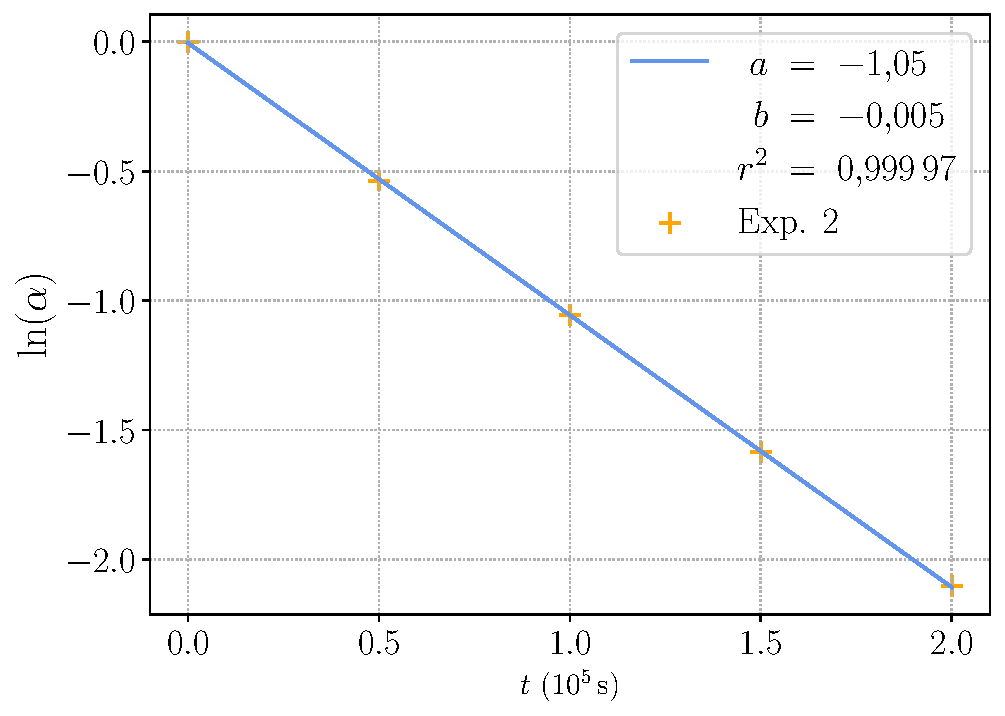
\includegraphics[width=\linewidth]{exo6_a1}
    \end{center}
\end{minipage}
}
\QR{%
  Déterminer la constante de vitesse de la réaction.
}{%
On obtient la constante de vitesse grâce à la pente de la régression
linéaire~:
\begin{gather*}
    -2k_{\rm app} = -2 k[\ce{Fe^{2+}}]_0
    \Leftrightarrow
    \boxed{
    k = \frac{2k_{\rm app}}{2[\ce{Fe^{2+}}]_0}}
    \qavec
    \left\{
        \begin{array}{rcl}
            2k_{\rm app} & = & \SI{1.051e-5}{s^{-1}}\\\relax
            [\ce{Fe^{2+}}]_0 & = & \SI{0.100}{mol.L^{-1}}
        \end{array}
    \right.\\
    \mathrm{A.N.~:}\quad
    \boxed{k = \SI{5.3e-5}{mol^{-1}.L.s^{-1}}}
\end{gather*}
}

\end{document}
